\documentclass[UTF8,10pt,a4paper]{ctexart}
\usepackage[margin=24mm]{geometry}
\usepackage{amsmath,amssymb,graphicx,booktabs,microtype,placeins,longtable}
\usepackage[colorlinks=true,linkcolor=blue,urlcolor=blue]{hyperref}
\setlength{\emergencystretch}{2em}
\graphicspath{{figures/}}
\renewcommand{\thesection}{S\arabic{section}}
\renewcommand{\thefigure}{S\arabic{figure}}
\renewcommand{\thetable}{S\arabic{table}}
\newcommand{\SteadyState}{稳态}
\newcommand{\SteadyCheck}{稳态模态核对}
\newcommand{\TransientCheck}{瞬态模态核对}
\newcommand{\RayCheck}{瞬态光路积分核对}
\title{补充材料1：斜入射加热圆柱光学元件的补充数值结果}
\author{Zhongwei Yang, Jing Wen, Wei Li, Tingrui Li, Bohui Chen, and Liang Yang}
\date{}
\begin{document}
\maketitle

\section{逐时刻的有限元与半解析结果比较}
表~\ref{tab:supp-comparison} 列出稳态以及每个记录时刻的比较结果，补充正文中只列最大值的汇总表。
其中，$0.001$ s 为早期诊断时刻；正文的瞬态最大值取自 $0.0025$--$75$ s。
表内数值均为百分数，归一化分母由半解析解提供。

温度列取前表面、中间截面和后表面中最大的相对最大差异。
在 $0.625$ s 之前，三个截面统一除以半解析解在这三个截面中的最大温升；此后，各截面除以自身的最大温升。
计算 OPD 场差异时，先分别减去两个场在共同光瞳内的平均值，再计算二者的 RMS 差异和最大差异。
这两项场差异以及 PV 的绝对差值，均除以半解析 OPD 的 PV。
稳态温度比较使用笛卡尔网格：$0^\circ$ 为 $201\times201$，$30^\circ$ 和 $60^\circ$ 为 $101\times101$。
瞬态温度比较使用 $201\times201$ 极坐标采样点，径向采用 Gauss 节点，方位角均匀分布。
三个角度的 OPD 比较均使用 $101\times101$ 笛卡尔入口网格。
共同光瞳仅保留能到达后表面、且位于有限元多边形内的光线。

\begingroup\small
\begin{longtable}{ccrrrr}
\caption{稳态及各时刻的有限元--半解析差异（\%）。三个 OPD 列依次为 RMS 差异/PV、最大差异/PV、PV 绝对差值/PV。}\label{tab:supp-comparison}\\
\toprule
入射角 & 状态／$t$（s） & 温度最大差异 & OPD RMS & OPD 最大差异 & OPD-PV\\\midrule
\endfirsthead
\multicolumn{6}{c}{表~\thetable（续）}\\\toprule
入射角 & 状态／$t$（s） & 温度最大差异 & OPD RMS & OPD 最大差异 & OPD-PV\\\midrule
\endhead
\bottomrule\endfoot
$0^\circ$ & \SteadyState & 0.031420 & 0.001417 & 0.005848 & 0.004220\\
$0^\circ$ & 0.001 & 0.117929 & 0.014570 & 0.092695 & 0.057930\\
$0^\circ$ & 0.0025 & 0.116871 & 0.014252 & 0.090254 & 0.071263\\
$0^\circ$ & 0.01 & 0.113496 & 0.014261 & 0.088373 & 0.055804\\
$0^\circ$ & 0.05 & 0.104563 & 0.014429 & 0.083029 & 0.025750\\
$0^\circ$ & 0.1 & 0.105207 & 0.014508 & 0.085021 & 0.015655\\
$0^\circ$ & 0.625 & 0.136599 & 0.013882 & 0.082121 & 0.006193\\
$0^\circ$ & 2.5 & 0.089698 & 0.011499 & 0.060701 & 0.014736\\
$0^\circ$ & 20 & 0.063480 & 0.006925 & 0.034443 & 0.019302\\
$0^\circ$ & 50 & 0.067147 & 0.010957 & 0.040858 & 0.040530\\
$0^\circ$ & 75 & 0.079316 & 0.011790 & 0.042388 & 0.043933\\
\midrule
$30^\circ$ & \SteadyState & 0.023794 & 0.001286 & 0.004131 & 0.000523\\
$30^\circ$ & 0.001 & 0.117743 & 0.013721 & 0.094190 & 0.041289\\
$30^\circ$ & 0.0025 & 0.116424 & 0.013329 & 0.083826 & 0.054396\\
$30^\circ$ & 0.01 & 0.112007 & 0.013258 & 0.080928 & 0.040434\\
$30^\circ$ & 0.05 & 0.099291 & 0.013105 & 0.083503 & 0.015371\\
$30^\circ$ & 0.1 & 0.099894 & 0.012872 & 0.085119 & 0.006973\\
$30^\circ$ & 0.625 & 0.128643 & 0.010799 & 0.077983 & 0.010758\\
$30^\circ$ & 2.5 & 0.081803 & 0.007949 & 0.050021 & 0.013332\\
$30^\circ$ & 20 & 0.057135 & 0.005355 & 0.025311 & 0.019177\\
$30^\circ$ & 50 & 0.070454 & 0.010840 & 0.033466 & 0.042286\\
$30^\circ$ & 75 & 0.082138 & 0.011756 & 0.035206 & 0.045718\\
\midrule
$60^\circ$ & \SteadyState & 0.111849 & 0.024332 & 0.071196 & 0.005436\\
$60^\circ$ & 0.001 & 0.103873 & 0.024675 & 0.095791 & 0.010805\\
$60^\circ$ & 0.0025 & 0.102273 & 0.024325 & 0.082575 & 0.004631\\
$60^\circ$ & 0.01 & 0.096810 & 0.024179 & 0.074261 & 0.002073\\
$60^\circ$ & 0.05 & 0.088028 & 0.023641 & 0.071822 & 0.016120\\
$60^\circ$ & 0.1 & 0.085548 & 0.022982 & 0.071356 & 0.021721\\
$60^\circ$ & 0.625 & 0.119119 & 0.017821 & 0.063808 & 0.021537\\
$60^\circ$ & 2.5 & 0.061998 & 0.010835 & 0.040743 & 0.010770\\
$60^\circ$ & 20 & 0.066121 & 0.007085 & 0.025537 & 0.017211\\
$60^\circ$ & 50 & 0.093480 & 0.012963 & 0.035470 & 0.043028\\
$60^\circ$ & 75 & 0.100718 & 0.013720 & 0.035250 & 0.046819\\

\end{longtable}
\endgroup
稳态行使用表~\ref{tab:supp-fem-settings} 中最细的稳态有限元网格；瞬态行使用正文的瞬态有限元配置。

\section{数值加密前后的实际变化}
这里的“加密”指增加级数中保留的项数、数值积分点数或有限元单元数。
它不改变基底尺寸、热载荷、波长或材料参数。
下面将每组计算的具体设置与所得变化一起列出。

\subsection*{半解析 OPD 的核对数据}
表~\ref{tab:supp-sa-settings} 中，$M$ 是保留的最高温度方位阶次，$N$ 是每个方位阶次保留的径向模态数，$J$ 是瞬态展开保留的轴向模态数。
$Q_r\times Q_\phi$ 是将热载荷投影到各模态时使用的径向、方位角积分点数，不是温度图的像素数。
$Q_s$ 是沿每条折射光线的积分点数，不是光线条数。

\begin{table}[!htbp]\centering\small
\caption{正文计算与 OPD 核对计算的具体设置。“--”表示稳态计算不使用瞬态轴向展开。}\label{tab:supp-sa-settings}
\begin{tabular}{lrrrrr}\toprule
计算组 & $M$ & $N$ & $J$ & $Q_r\times Q_\phi$ & $Q_s$\\\midrule
正文稳态计算 & 6 & 8 & -- & $400\times32$ & 16\\
稳态模态核对 & 10 & 20 & -- & $1200\times128$ & 32\\
正文瞬态计算 & 10 & 20 & 256 & $1200\times128$ & 32\\
瞬态模态核对 & 14 & 28 & 384 & $1800\times256$ & 64\\
仅增加瞬态光路积分点 & 10 & 20 & 256 & $1200\times128$ & 64\\\bottomrule
\end{tabular}
\end{table}

表~\ref{tab:supp-sa-changes} 给出正文计算与对应核对计算之间的变化。
稳态部分在每个入射角下比较一次；瞬态部分取表~\ref{tab:supp-comparison} 中十个正时刻内的最大变化。
这些光学核对统一采用 $101\times101$ 的物理透射光瞳采样。
各列均以核对计算的 OPD-PV 归一化，计算场差异前去除活塞项。
因此，表中数值表示两组数值设置之间的变化，而不是相对于精确解的误差。

\begin{table}[!htbp]\centering\small
\caption{表~\ref{tab:supp-sa-settings} 中各组核对得到的 OPD 变化（\%）。}\label{tab:supp-sa-changes}
\begin{tabular}{lrrrr}\toprule
比较项目 & 入射角 & PV 变化 & RMS/PV & 最大差异/PV\\\midrule
\SteadyCheck & $0^\circ$ & 0.009586 & 0.001011 & 0.008559\\
\SteadyCheck & $30^\circ$ & 0.005571 & 0.000651 & 0.005044\\
\SteadyCheck & $60^\circ$ & 0.010106 & 0.024238 & 0.063912\\
\midrule
\TransientCheck & $0^\circ$ & 0.016817 & 0.002829 & 0.016207\\
\TransientCheck & $30^\circ$ & 0.016821 & 0.003038 & 0.016629\\
\TransientCheck & $60^\circ$ & 0.044419 & 0.019406 & 0.052442\\
\midrule
\RayCheck & $0^\circ$ & 0.018206 & 0.002863 & 0.017192\\
\RayCheck & $30^\circ$ & 0.018212 & 0.003070 & 0.017021\\
\RayCheck & $60^\circ$ & 0.018215 & 0.003962 & 0.015952\\\bottomrule

\end{tabular}
\end{table}
温度场与温度梯度的截断核对采用表~\ref{tab:supp-temperature-settings} 中另外两组配置。
A、B 是同一热问题的两组有限数值参考；B 组保留更多展开项，同时增加热源投影的积分点数。
这张表补充正文提到的温度参考设置；表~\ref{tab:supp-sa-settings} 则列出当前 OPD 核对所用的设置。

\begin{table}[!htbp]\centering\small
\caption{温度场核对采用的两组参考配置。$M$、$N$、$J$ 和热源投影积分点数的含义同上。}\label{tab:supp-temperature-settings}
\begin{tabular}{lrrrr}\toprule
温度计算 & $M$ & $N$ & $J$ & $Q_r\times Q_\phi$\\\midrule
稳态参考 A & 14 & 32 & -- & $2400\times256$\\
稳态参考 B & 16 & 40 & -- & $3200\times512$\\
瞬态参考 A & 14 & 32 & 512 & $2400\times256$\\
瞬态参考 B & 16 & 40 & 768 & $3200\times512$\\\bottomrule
\end{tabular}
\end{table}

\FloatBarrier

\subsection*{有限元温度场的核对数据}
表~\ref{tab:supp-fem-settings} 明确列出空间加密时改变的网格。
稳态与瞬态采用相同的横向网格；稳态轴向网格均匀分布，瞬态轴向网格在两个端面附近加密。
仅检查时间步长时，保持正文瞬态网格不变，将每个时间步减半，总步数由 $2176$ 增至 $4352$。
瞬态联合加密同时采用更细的横向网格、轴向网格和减半的时间步长。

\begin{table}[!htbp]\centering\small
\caption{有限元温度加密比较所用网格。总自由度指完整计算空间的自由度数。}\label{tab:supp-fem-settings}
\begin{tabular}{lrrrrr}\toprule
 & 横向 & \multicolumn{2}{c}{稳态} & \multicolumn{2}{c}{瞬态}\\
配置 & 自由度 & 轴向单元数 & 总自由度 & 轴向单元数 & 总自由度\\\midrule
正文网格 & 2113 & 32 & 137345 & 88 & 374001\\
仅横向加密 & 8321 & 32 & 540865 & 88 & 1472817\\
仅轴向加密 & 2113 & 64 & 272577 & 174 & 737437\\
横向与轴向加密 & 8321 & 64 & 1073409 & 174 & 2904029\\\bottomrule
\end{tabular}
\end{table}
正文瞬态计算在相邻观测时刻之间采用 $128$ 个时间步，只有 $0.1$--$0.625$ s 区间采用 $1024$ 步。
从 $0$ 到 $75$ s 共计 $2176$ 步。

图~\ref{fig:supp-fem-refinement} 给出正文最大值所对应的逐时刻温度加密结果。
每条曲线在每个时刻，取三个固定截面和七个扩散深度采样中的最大相对 $L^2$ 差异或最大相对温度差异。
在 $0.625$ s 之前，各范数除以上述深度中最大的对应加密参考范数；此后，各深度使用自身的参考范数。
这些曲线比较的是有限元温度场加密前后的变化；表~\ref{tab:supp-comparison} 的光学列比较的则是有限元与半解析两种方法。

\begin{figure}[!htbp]\centering
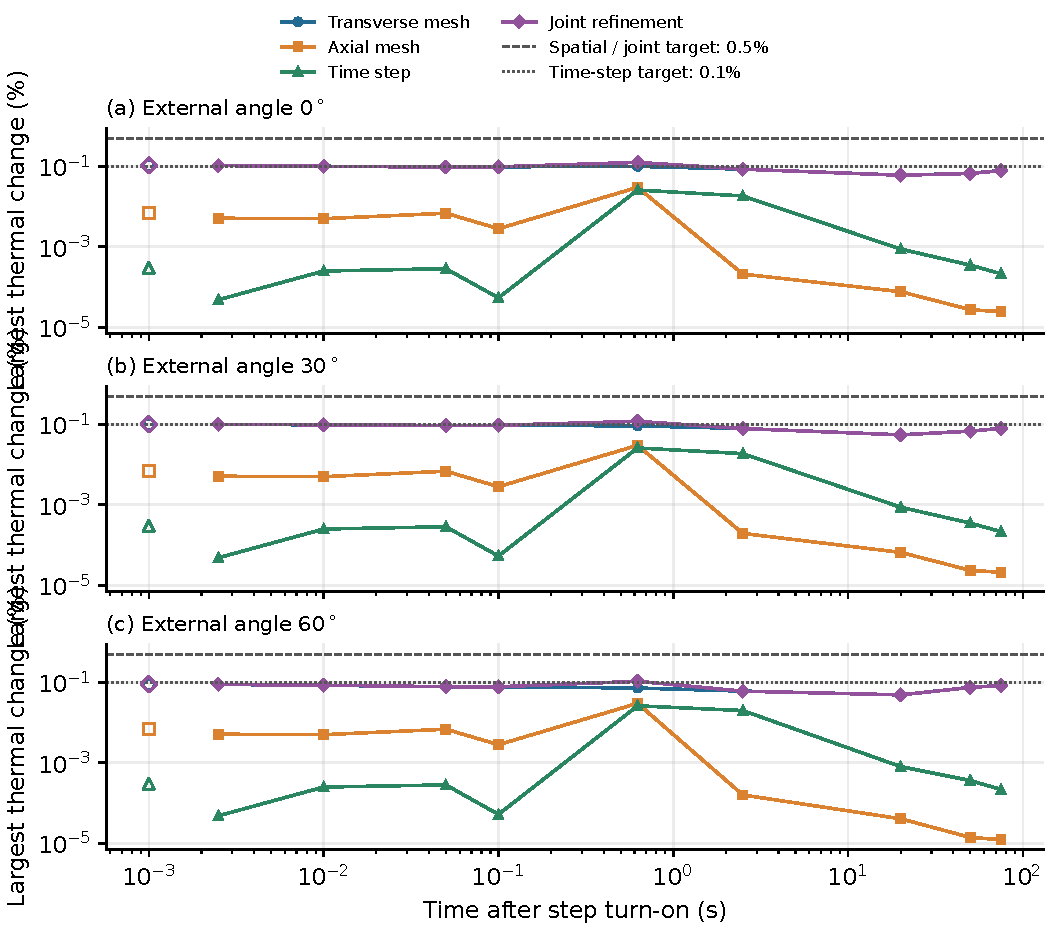
\includegraphics[width=.91\linewidth]{supp_transient_fem_refinement.pdf}
\caption{$0^\circ$、$30^\circ$、$60^\circ$ 下，横向网格、轴向网格、时间步长及联合加密引起的温度变化。
实心点覆盖 $0.0025$--$75$ s；未连线的空心点为 $0.001$ s 诊断结果。
虚线和点线分别为 $0.5\%$ 的空间／联合加密目标与 $0.1\%$ 的时间步长加密目标。}
\label{fig:supp-fem-refinement}
\end{figure}
\FloatBarrier

\section{补充 OPD 数值与稳态场对比}
表~\ref{tab:supp-pupil-pv} 对照正文所用的物理光瞳网格采样值与连续光瞳极值估计。
前者使用保存的 $201\times201$ 笛卡尔网格，并仅保留物理透射光瞳内的点。
后者在同一物理光瞳上采用多起点 SLSQP 数值寻优；改变的是寻找最大值和最小值的方式，而不是温度解或光学参数。
最后一列为“连续极值估计减去网格采样值”，单位为 nm，不是有限元误差。
差值由未舍入的数值计算。

\begin{table}[!htbp]\centering\small
\caption{网格采样与连续光瞳估计所得的 OPD-PV（nm）。}\label{tab:supp-pupil-pv}
\begin{tabular}{lrrrr}\toprule
状态／时刻 & 入射角 & 网格 PV & 连续估计 PV & 差值\\\midrule
\SteadyState & $0^\circ$ & 145.9575 & 145.9575 & 0.0000\\
\SteadyState & $30^\circ$ & 147.9398 & 147.9727 & 0.0329\\
\SteadyState & $60^\circ$ & 135.0684 & 135.0748 & 0.0065\\
\midrule
0.625 s & $0^\circ$ & 13.0804 & 13.0804 & 0.0000\\
0.625 s & $30^\circ$ & 12.2102 & 12.2121 & 0.0019\\
0.625 s & $60^\circ$ & 8.5015 & 8.5021 & 0.0006\\
\midrule
75 s & $0^\circ$ & 137.0548 & 137.0548 & 0.0000\\
75 s & $30^\circ$ & 137.5772 & 137.5924 & 0.0153\\
75 s & $60^\circ$ & 123.3885 & 123.3909 & 0.0024\\\bottomrule

\end{tabular}
\end{table}

正文给出了瞬态场对比，图~\ref{fig:steadyfem} 补充 $60^\circ$ 入射时的稳态空间对比。
每一行中的两种方法使用相同的公共采样点，两个场共用色标。

\begin{figure}[!htbp]\centering
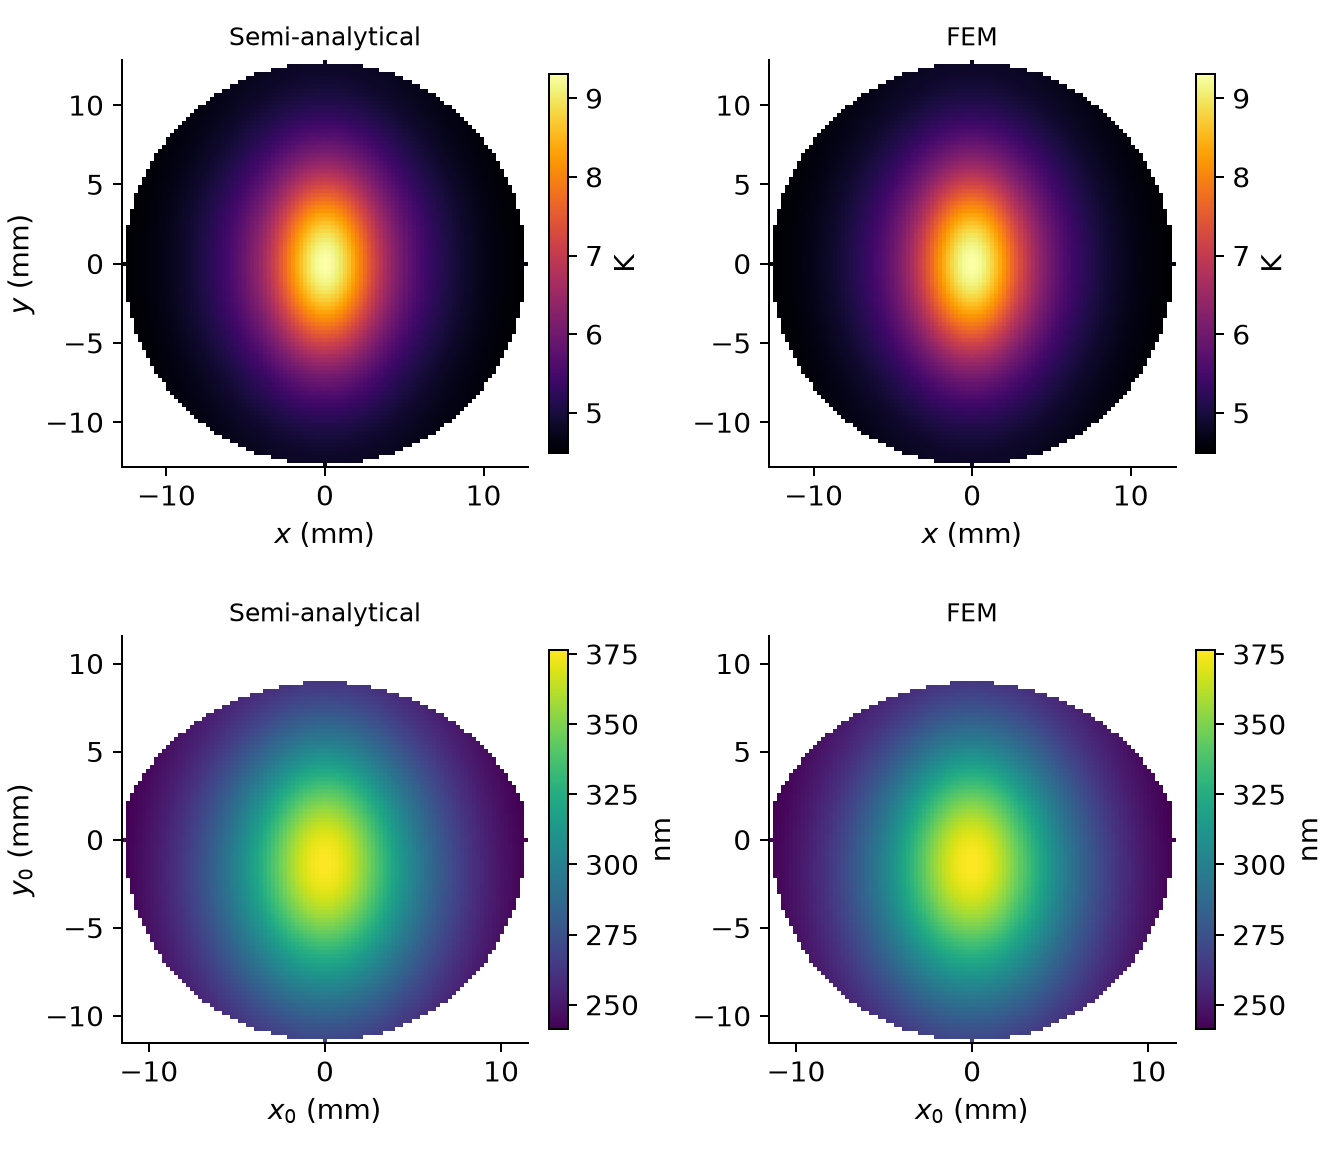
\includegraphics[width=.74\linewidth]{steady_fem_comparison.png}
\caption{$60^\circ$ 稳态对比：左列为半解析场，右列为最细有限元场。
上行为前表面温升，下行为公共光瞳上的折射光路 OPD。
每一行中的两个场共用色标。}
\label{fig:steadyfem}
\end{figure}
\FloatBarrier
\end{document}
